\documentclass[10pt]{beamer}

%%%
% PREAMBLE FOR THIS DOC 
%%%
%https://tex.stackexchange.com/questions/68821/is-it-possible-to-create-a-latex-preamble-header
\usepackage{/Users/miw267/Repos/csci246_spring2025/slides/preambles/beamer_preamble_for_CSCI246}



%%% TRY TO RESHOW TOC AT EACH SECTION START (with current section highlighted)
% Reference: https://tex.stackexchange.com/questions/280436/how-to-highlight-a-specific-section-in-beamer-toc
\newcommand\tocforsect[2]{%
  \begingroup
  \edef\safesection{\thesection}
  \setcounter{section}{#1}
  \tableofcontents[#2,currentsection]
  \setcounter{section}{\safesection}
  \endgroup
}


%%%% HERES HOW TO DO IT CORRECTLY
% FIRST IN .STY FILE, DO
%\usetheme[sectionpage=none]{metropolis}
% THEN AT EACH SECTION DO
%\begin{frame}{Outline}
%  \tableofcontents[currentsection]	
%\end{frame}



%\setbeamertemplate{navigation symbols}{}
%\setbeamertemplate{footline}[frame number]{}


%%%
% DOCUMENT
%%%

\begin{document}

%\maketitle

%% Title page frame
%\begin{frame}
%    \titlepage 
%\end{frame}





\title{02/19/2025: Introduction to Relations}
\author{CSCI 246: Discrete Structures}
\date{Textbook reference: Ch 11.1-11.2, Hampkins}

\begin{frame}
    \titlepage 
\end{frame}


\begin{frame}
\footnotesize 
\begin{mygreenbox}[title=Graded Quiz Pickup]
Quizzes are in the front of the room, grouped into four bins (A-G, H-L, M-R, S-Z) by last name. The quizzes are upside down with your last name on the back. Come find yours before, during, or after class.  Only turn the quiz over if it's yours.
\end{mygreenbox} 
\vfill 

%\begin{myredbox}[title=Announcements]
%
%\begin{itemize}
%\item Wednesday's reading quiz was graded out of 1 point.  45/60 students who took the quiz scored 100\%.
%\item Note: The reading quizzes are equally weighted.  The denominator is typically chosen for convenience.  
%\end{itemize}
%
%\end{myredbox}
%
%\vfill 


\begin{myyellowbox}[title=Today's Agenda]
\begin{itemize}
	\item Reading quiz (5 mins)
	\item Mini-lecture ($\approx$ 20 mins)
%	%
%	\begin{itemize}
%	\footnotesize 
%	\item Review induction 
%	\end{itemize}
%	%
	\item Group exercises ($\approx$ 20 mins)
\end{itemize}

\end{myyellowbox}
\vfill 

\end{frame}




\begin{frame}
 

 \begin{mygreenbox}[title=Definition]
Suppose that $R$ is a binary relation on a set $A$.
\begin{enumerate}
	\item The relation $R$ is \textbf{reflexive} on $A$ if $a\,R\,a$ for all $a \in A$.
	\item  The relation $R$ is \textbf{symmetric} on $A$ if, whenever $a\,R\,b$, then also $b\,R\,a$.
	\item The relation $R$ is \textbf{transitive} on $A$ if, whenever $a\,R\,b$ and $b\,R\,c$, then also $a\,R\,c$.
\end{enumerate}
\end{mygreenbox}


 \vfill

 \begin{myredbox}[title=Reading Quiz (Relations)]
Give an example of 
\begin{enumerate}
	\item A binary relation that is reflexive and symmetric but not transitive.
	\item A binary relation that is reflexive and transitive but not symmetric.
	\item A binary relation that is symmetric and transitive but not reflexive.
\end{enumerate}
\end{myredbox}



\end{frame}


\begin{frame}[standout]
Notes on relations
\end{frame}


\begin{frame}
\footnotesize 
\begin{mygreenbox}[title=Definition]
Let $A$ and $B$ be two sets.  A \textbf{binary relation} (or simply a \textbf{relation}) $R$ from $A$ to $B$ is a subset of the Cartesian product $A \times B$.
\end{mygreenbox}

\begin{myredbox}[title=Example]
Let $A = \set{2,3,4,5,6}$ and $B=\set{3,6,9}$ and relation $R=\set{(a,b): a|b, a \in A, b \in B}$.  Then  $R= \set{(2,6), (3,3), (3,6), (3,9), (6,6)}$.

\begin{figure}
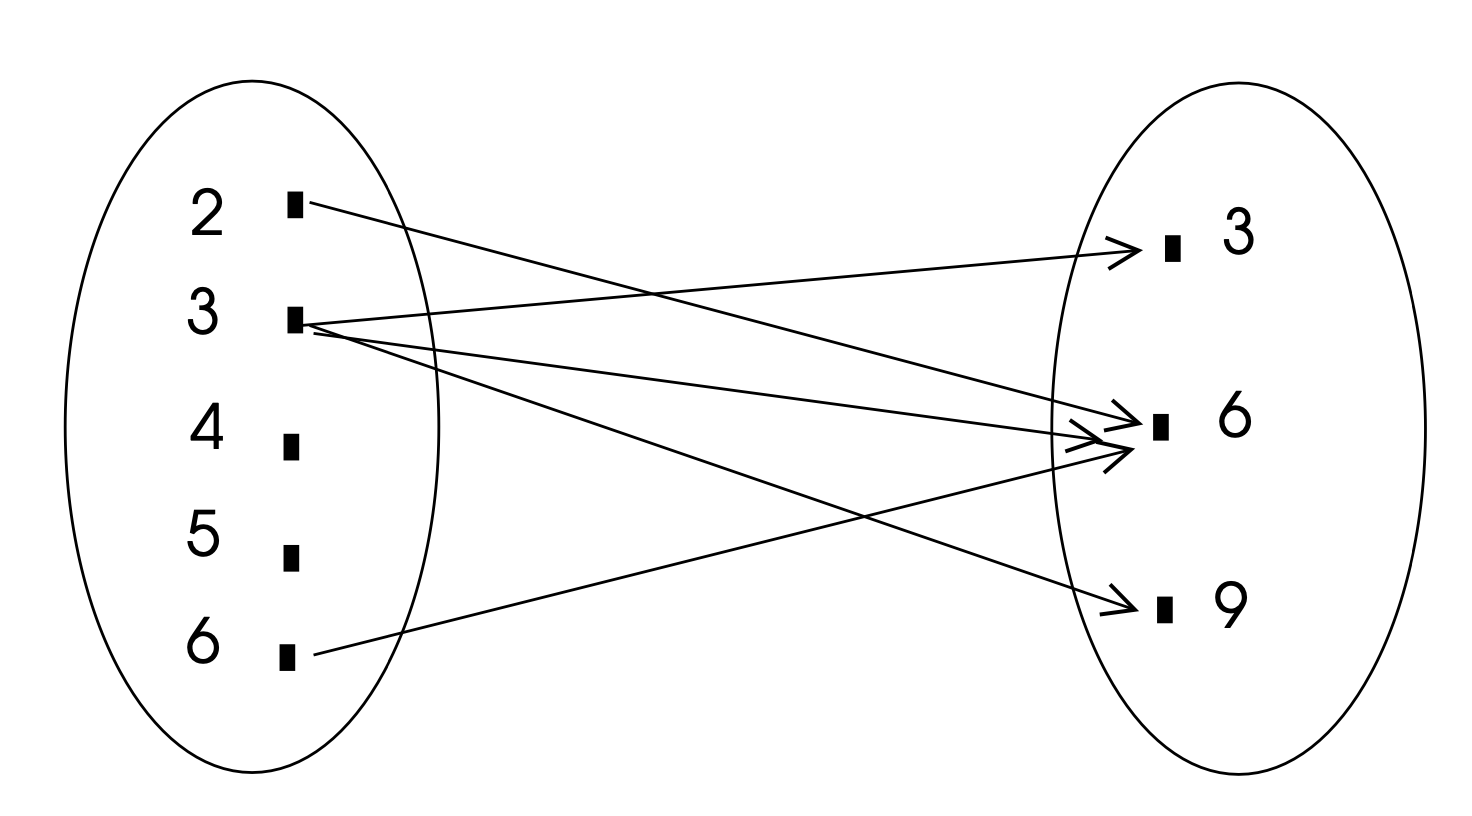
\includegraphics[width=.5\textwidth]{images/relation_example.png}	
\caption{Set diagram representation of the relation $R$}
\end{figure}

\end{myredbox}

\vfill 
\pause 
\begin{myyellowbox}[title=Poll]
Can this relation be reflexive, symmetric, and/or transitive? Why or why not?
\end{myyellowbox}

%relation_example
	
\end{frame}



\begin{frame}

\footnotesize 
\begin{myredbox}[title=Remark]
The reading considers relations where the two underlying sets are the same.  That is, it considers relations $R$ from $A$ to $A$, where  $A$ is a set.  Hence, the definitions of reflexive, symmetric, and transitive are relevant.
\end{myredbox}
\vfill 
\begin{myyellowbox}[title=Poll]
Now consider the relation $R=\set{(a,b): a|b}$ on the set $\mathbb{Z}$ of integers. 

Is this relation 
\begin{itemize}
\item Reflexive? \pause \greencheck Every number divides itself: $a|a$, since $a \cdot 1 = a$.
\item Symmetric? \pause \redx  For example, $3|6$ but it is not the case that $6|3$.
\item Transitive? \pause \greencheck    Suppose $a|b$ and $b|c$.  We need to show $a|c$.  Since $a|b$, there is an integer $q$ such that $b=aq$.  By definition of $b|c$, there is an integer $r$ such that $c=br$.  Hence we have 
\[ c=br = (aq)r = a(qr)\]
Hence there is an integer $s=qr$ such that $c=as$.  Hence $a|c$.  	
\end{itemize}
\end{myyellowbox}


\end{frame}



\begin{frame}{Example of Relations in Computer Science}
\footnotesize 
\begin{mygreenbox}[title=Example]

Let's consider a ``friendship" relation in a \textbf{social network} like Facebook. We can define a relation $R$ on a set of users where: $(x,y) \in R$ if and only if $x$ is a friend of $y$. 
\end{mygreenbox}

\begin{myyellowbox}[title=Poll]
Is this relation
\begin{itemize}
\item Reflexive? \pause \redx Users don't usually friend themselves in social networks. 
\item Symmetric? \pause \greencheck(-ish.) In most social networks, a friendship connection is bidirectional. If Alice is a friend of Bob, then Bob is a friend of Alice.  However, in platforms like X (formerly Twitter), where following is \textit{one-way}, the "follows" relation is \textit{not symmetric}.
\item Transitive? \pause \redx If  Alice is friends with Bob and Bob is friends with Charlie, it does not necessarily mean that Alice is friends with Charlie.  %However, in certain recommendation systems, the transitive property may be used to suggest friends-of-friends.
\end{itemize}
\end{myyellowbox}
	
\end{frame}


\begin{frame}

\begin{mygreenbox}[title=Why do relations matter?: Some examples from social networks]

\begin{itemize}
\item \textbf{Social Influence \& Virality}

\begin{itemize}
\item If relationships in a network are \alert{transitive}, messages, trends, and viral content can spread faster.
\end{itemize}

\item \textbf{Friend-of-a-Friend Recommendations}  
\begin{itemize}
\item Even if friendship is not strictly \alert{transitive}, many recommendation algorithms use approximate transitivity to suggest new friends (e.g., LinkedIn’s "People You May Know" feature).
\end{itemize}


\item \textbf{Algorithm Optimization}
\begin{itemize}
\item If a relation is \alert{symmetric}, storage can be optimized by only storing one direction of the connection.
\item Search algorithms (e.g., shortest path) can be optimized by reducing redundant checks.
\end{itemize}
\end{itemize}
\end{mygreenbox}

\end{frame}

\begin{frame}{Equivalence relations}
\begin{myredbox}[title=Definition]
An \textbf{equivalence relation} is a relation that is
\begin{enumerate}
\item Reflexive \greencheck
\item Symmetric \greencheck
\item Transitive \greencheck
\end{enumerate}
\end{myredbox}

\end{frame}


\begin{frame}
\footnotesize 
\begin{myredbox}[title=Remark]
\textbf{Q:} Why do equivalence relations matter?  \\
\pause 
\textbf{A:} They can make problem solving easier.
\end{myredbox}
\end{frame}

\begin{frame}
\footnotesize 
\begin{myredbox}[title=Remark]
\textbf{Q:} Why do equivalence relations matter?  \\
\textbf{A:} They can make problem solving easier.
\end{myredbox}

\vfill
\begin{mygreenbox}[title=Example]
\textbf{Q:} Why is $n^{70} - n^{22}$ always even? \\

\pause 
\textbf{Useful Point-Of-View (POV):} Let us define the "mod-2" equivalence relation (written $\equiv_2$).  Here two numbers are equivalent if they have the same remainder when divided by 2.  So
%
\begin{align*}
	x  \equiv_2 
	\begin{cases}
0, & \text{ if $x$ is even} \\
1, & \text{ if $x$ is odd}
	\end{cases}
\end{align*}
%
%(That is, all even numbers are equivalent to 0 and all odd numbers are equivalent to 1.)  \\
Now multiplication and addition is well-defined mod-2. (For justification, see Hampkins Ch2 or today's group exercises). So we can just use "0" and "1" as representatives in any multiplication or addition problem about odds and evens. \\

\pause 
\textbf{A:} By the above POV, we only need to consider two cases:
\begin{align*}
	n^{70} - n^{22} &= 0^{70} - 0^{22} =0-0 = 0 && \text{ if $n=0$ ($n$ is even)}\\
	n^{70} - n^{22} &= 1^{70} - 1^{22} =1-1 = 0 && \text{ if $n=1$ ($n$ is odd)}
\end{align*}
Either way, the result is 0 (the result is even).

\end{mygreenbox}

\end{frame}


\begin{frame}{Take home}
\footnotesize 
\begin{myredbox}[title= The purpose of equivalences]
The purpose of equivalences is similar to the purpose of the set identities we did last class: they can help us see things from different perspectives.  \\
\vfill 
Whether it's looking at each side of an equality of an identity, or  creatively constructing  new equivalence relations, these tools can help us to solve problems that  aren't otherwise solvable (quickly or at all).
	
\end{myredbox}

\vfill \vfill 
\pause 
\begin{myyellowbox}[title= The purpose of multiple points of view]
Why see things from different points of view?  Recall from Hampkins Ch2 (Multiple Proofs), different points of view suggest different generalizations. \\
\vfill 
For example, consider how hard it would be to answer the question about $n^{70}-n^{22}$ if, instead of using mod-2 equivalences, we tried the extending the picture proof we used for $n^2-n$: 
\begin{center}
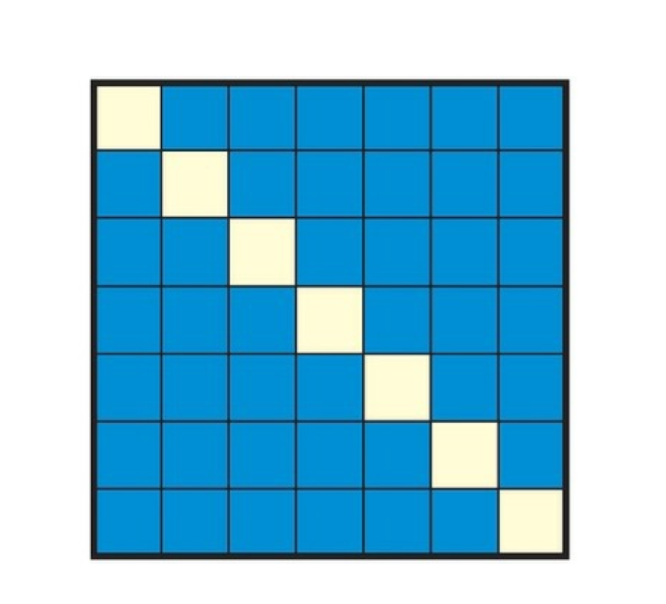
\includegraphics[width=.2\textwidth]{images/n_squared_minus_n}	
\end{center}

\end{myyellowbox}



	
\end{frame}


\begin{frame}
\footnotesize
Group 1: erik.moore3,samuel.hemmen,julia.larsen\\
Group 2: jacob.shepherd1,connor.graville,luke.donaldson1\\
Group 3: derek.price4,griffin.short,luka.derry\\
Group 4: cameron.wittrock,tristan.nogacki,jack.fry\\
Group 5: connor.yetter,conner.reed1,john.fotheringham\\
Group 6: james.brubaker,caitlin.hermanson,devon.maurer\\
Group 7: pendleton.johnston,evan.schoening,adam.wyszynski\\
Group 8: timothy.true,blake.leone,joseph.mergenthaler\\
Group 9: jonas.zeiler,anthony.mann,colter.huber\\
Group 10: justice.mosso,carver.wambold,peter.buckley1\\
Group 11: aaron.loomis,nolan.scott1,sarah.periolat\\
Group 12: matthew.nagel,samuel.rollins,carsten.brooks\\
Group 13: owen.obrien,ryan.barrett2,jett.girard\\
Group 14: samuel.mosier,tyler.broesel,evan.barth\\
Group 15: jacob.ruiz1,delaney.rubb,peyton.trigg\\
Group 16: zeke.baumann,yebin.wallace,mason.barnocky\\
Group 17: jeremiah.mackey,alexander.goetz,bridger.voss\\
Group 18: lucas.jones6,reid.pickert,jakob.kominsky\\
Group 19: emmeri.grooms,kaden.price,william.elder1\\
Group 20: jacob.ketola,lynsey.read,connor.mizner\\
Group 21: joseph.triem,michael.oswald,micaylyn.parker\\
Group 22: alexander.knutson,ethan.johnson18,jada.zorn\\
\end{frame}


\begin{frame}{Group Exercises: Introduction to Relations}

\begin{enumerate}
	\item Consider the collection of numerical expressions for rational numbers, like $\frac{3}{4}$ or $-\frac{6}{12}$.  Let us consider these expressions not as numbers but as syntactic expressions $\frac{p}{q}$ -- that is,  as pairs of integers, a numerator $p$ and nonzero denominator $q$ -- so that we count $\frac{1}{2}$ as a different expression than $\frac{2}{4}$.  Define the relation $\frac{p}{q} \approx \frac{r}{s}$ for such expressions if they represent the same rational number, which happens precisely when $ps=rq$ in the integers.  Prove this is an equivalence relation. 
	\item A relation $R$ is defined on $\mathbb{Z}$ by $a\,R\,b$ if $a+b$ is even.  Show that $R$ is an equivalence relation.
	\item (Bonus.) Show that both addition and multiplication are well-defined with respect to congruence modulo $n$, for every positive integer $n$.
\end{enumerate}

\end{frame}


\begin{frame}{Solution to Group Exercise \#1} 
\small 
\textbf{Solution.}  We verify the three properties of an equivalence relationship below.

\begin{itemize}
\item \textit{Reflexivity}:  We need to check
\[ \frac{p}{q} \approx \frac{p}{q},  \]
which happens when $pq=pq$. This is always true. \greencheck.
\item \textit{Symmetry}: We need to check that if $\frac{p}{q} \approx \frac{r}{s}$ , then $\frac{r}{s} \approx \frac{p}{q}$.  That is, we need to check that if $ps=qr$, then $rq=sp$. This is true by commutativity of multiplication. \greencheck.
\item \textit{Transitivity}: We need to check that if  $\frac{p}{q} \approx \frac{r}{s}$  and $\frac{r}{s} \approx \frac{t}{u}$, then $\frac{p}{q} \approx \frac{t}{u}$.  That is, we need to check that if $ps=qr$ and $ru=st$, then $pu=qt$.  Now note
\begin{align*}
ps &=qr && \scripttext{By hypothesis} \\
ps(ru) &=qr(st) && \scripttext{Multiply both sides by same amount} \\
p\cancel{s}(\cancel{r}u) &=q\cancel{r}(\cancel{s}t) && \scripttext{Cancel identical terms} \\
pu &=qt, 	
\end{align*}
which is what we needed to show.  \greencheck
\end{itemize}


\end{frame}


\begin{frame}{Solution to Group Exercise \#2} 
\small 
\textbf{Problem.} A relation $R$ is defined on $\mathbb{Z}$ by $a\,R\,b$ if $a+b$ is even.  Show that $R$ is an equivalence relation.
\vfill 
\textbf{Solution.} We verify the three properties of an equivalence relationship below.


\begin{itemize}
\item \textit{Reflexivity}:  We need to check $aRa$, which means that $a+a$ must be even. But $a+a=2a$, which is even by definition of even. \; \greencheck
\item \textit{Symmetry}: We need to check that if $aRb$ , then $bRa$.  That is, we need to check that if $a+b$ is even, then $b+a$ is even. This is true by commutativity of addition. \; \greencheck
\item \textit{Transitivity}:  We need to check that if $aRb$ and $bRc$ , then $aRc$.   That is, we need to check that if $a+b$ and $b+c$ are even, then $a+c$ is even.  Now by definition of even, $a+b=2q$ and $b+c=2r$ for some integers $q$ and $r$.  Thus
\begin{align*}
(a+b) + (b+c) &= 2q+2r \\
\implies a+2b+c &= 2q+2r \\
\implies a+c &= 2q+2r -2b = 2(q+r-b),	
\end{align*}
and so $a+c$ is even by the definition of even. \greencheck
\end{itemize}
\end{frame}

\begin{frame}{Solution to Group Exercise \#3} 
\small 
\textbf{Problem (Bonus.)} Show that both addition and multiplication are well-defined with respect to congruence modulo $n$, for every positive integer $n$.
\vfill 
\textbf{Remark 1.} By definition of congruence modulo $n$, if $x \equiv_n x'$, then $x=x' + nr$ for some integer $r$.
\vfill 
\textbf{Solution to problem.}  Suppose $x \equiv_n x'$ and $y \equiv_n y'$.  Then by Remark 1, $x=x' + nr$ for some integer $r$ and $y=y' + nq$ for some integer $q$. Now note
%
\begin{align*}
x+y &= x' + y' + nr+ nq \\
&= x' +y' + n(r+q)	
\end{align*}
Hence  $x+y \equiv_n x'+y'$. \greencheck 

Moreover,
\begin{align*}
xy &= (x' +nr) (y' + nq) \\
&= x'y' + x'nq + y'nr + n^2rq \\
&= x'y' + n(x'q + y'r + nrq)	
\end{align*}
Hence  $xy \equiv_n x'y'$. \greencheck 

\vfill 
\textbf{Remark 2.} This problem generalizes Thm. 88 on pp.124 of  Hampkins. 

\end{frame}
\end{document}
